\documentclass[10pt]{article}
\usepackage[utf8]{inputenc}
\usepackage[T1]{fontenc}
\usepackage{amsmath}
\usepackage{amsfonts}
\usepackage{amssymb}
\usepackage[version=4]{mhchem}
\usepackage{stmaryrd}
\usepackage{bbold}
\usepackage{graphicx}
\usepackage[export]{adjustbox}
\graphicspath{ {./images/} }

\begin{document}
\section*{FINAL JEE-MAIN EXAMINATION - JANUARY, 2023 \\
 (Held On Wednesday \(\mathbf{2 5}^{\text {th }}\) January, 2023) \\
 TIME:9:00 AM to 12: 00 NOON}
\section*{MATHEMATICS}
\section*{SECTION-A}
\begin{enumerate}
  \setcounter{enumi}{60}
  \item Let M be the maximum value of the product of two positive integers when their sum is 66 . Let the sample space \(S=\left\{x \in Z: x(66-x) \geq \frac{5}{9} M\right\}\) and the event \(\mathrm{A}=\{\mathrm{x} \in \mathrm{S}: \mathrm{x}\) is a multiple of 3\(\}\). Then \(\mathrm{P}(\mathrm{A})\) is equal to\\
(1) \(\frac{15}{44}\)\\
(2) \(\frac{1}{3}\)\\
(3) \(\frac{1}{5}\)\\
(4) \(\frac{7}{22}\)
\end{enumerate}

Official Ans. by NTA (2)\\
Allen Ans. (2)\\
Sol. \(\mathrm{M}=33 \times 33\)\\
\(x(66-x) \geq \frac{5}{9} \times 33 \times 33\)\\
\(11 \leq x \leq 55\)\\
A : \(\{12,15,18\),\\
54\}\\
\(\mathrm{P}(\mathrm{A})=\frac{15}{45}=\frac{1}{3}\)\\
62. Let \(\vec{a}, \vec{b}\) and \(\vec{c}\) be three non zero vectors such that \(\vec{b} \cdot \vec{c}=0\) and \(\vec{a} \times(\vec{b} \times \vec{c})=\frac{\vec{b}-\vec{c}}{2}\). If \(\vec{d}\) be a vector such that \(\vec{b} \cdot \vec{d}=\vec{a} \cdot \vec{b}\), then \((\vec{a} \times \vec{b}) \cdot(\vec{c} \times \vec{d})\) is equal to\\
(1) \(\frac{3}{4}\)\\
(2) \(\frac{1}{2}\)\\
(3) \(-\frac{1}{4}\)\\
(4) \(\frac{1}{4}\)

Official Ans. by NTA (4)\\
Allen Ans. (4)\\
Sol. \((\vec{a} \cdot \vec{c}) \vec{b}-(\vec{a} \cdot \vec{b}) \vec{c}=\frac{\vec{b}-\vec{c}}{2}\)\\
\(\vec{a} \cdot \vec{c}=\frac{1}{2}, \vec{a} \cdot \vec{b}=\frac{1}{2}\)\\
\(\therefore \overrightarrow{\mathrm{b}} \cdot \overrightarrow{\mathrm{d}}=\frac{1}{2}\)

\section*{TEST PAPER WITH SOLUTION}
\((\vec{a} \times \vec{b}) \cdot(\vec{c} \times \vec{d})=\vec{a} \cdot(\vec{b} \times(\vec{c} \times \vec{d}))\)\\
\(=\vec{a} \cdot((\vec{b} \cdot \vec{d}) \vec{c}-(\vec{b} \cdot \vec{c}) \vec{d})\)\\
\(=(\overrightarrow{\mathrm{a}} \cdot \overrightarrow{\mathrm{c}})(\overrightarrow{\mathrm{b}} \cdot \overrightarrow{\mathrm{d}})=\frac{1}{4}\)\\
63. Let \(y=y(x)\) be the solution curve of the differential equation \(\frac{d y}{d x}=\frac{y}{x}\left(1+x y^{2}\left(1+\log _{e} x\right)\right)\), \(x>0, y(1)=3\). Then \(\frac{y^{2}(x)}{9}\) is equal to :\\
(1) \(\frac{x^{2}}{5-2 x^{3}\left(2+\log _{e} x^{3}\right)}\)\\
(2) \(\frac{x^{2}}{2 x^{3}\left(2+\log _{e} x^{3}\right)-3}\)\\
(3) \(\frac{x^{2}}{3 x^{3}\left(1+\log _{e} x^{2}\right)-2}\)\\
(4) \(\frac{x^{2}}{7-3 x^{3}\left(2+\log _{e} x^{2}\right)}\)

Official Ans. by NTA (1)\\
Allen Ans. (1)\\
Sol. \(\frac{d y}{d x}-\frac{y}{x}=y^{3}\left(1+\log _{e} x\right)\)\\
\(\frac{1}{\mathrm{y}^{3}} \frac{\mathrm{dy}}{\mathrm{dx}}-\frac{1}{\mathrm{xy}^{2}}=1+\log _{\mathrm{e}} \mathrm{x}\)\\
Let \(-\frac{1}{\mathrm{y}^{2}}=\mathrm{t} \Rightarrow \frac{2}{\mathrm{y}^{3}} \frac{\mathrm{dy}}{\mathrm{dx}}=\frac{\mathrm{dt}}{\mathrm{dx}}\)\\
\(\therefore \frac{\mathrm{dt}}{\mathrm{dx}}+\frac{2 \mathrm{t}}{\mathrm{x}}=2\left(1+\log _{\mathrm{e}} \mathrm{x}\right)\)\\
I.F. \(=\mathrm{e}^{\int \frac{2}{\mathrm{x}} \mathrm{dx}}=\mathrm{x}^{2}\)\\
\(\frac{-x^{2}}{y^{2}}=\frac{2}{3}\left(\left(1+\log _{e} x\right) x^{3}-\frac{x^{3}}{3}\right)+C\)\\
\(y(1)=3\)\\
\(\frac{y^{2}}{9}=\frac{x^{2}}{5-2 x^{3}\left(2+\log _{e} x^{3}\right)}\)\\
OR

\[
\begin{aligned}
& x d y=y d x+x y^{3}\left(1+\log _{e} x\right) d x \\
& \frac{x d y-y d x}{y^{3}}=x\left(1+\log _{e} x\right) d x \\
& -\frac{x}{y} d\left(\frac{x}{y}\right)=x^{2}\left(1+\log _{e} x\right) d x \\
& -\left(\frac{x}{y}\right)^{2}=2 \int x^{2}\left(1+\log _{e} x\right) d x
\end{aligned}
\]

\begin{enumerate}
  \setcounter{enumi}{63}
  \item The value of
\end{enumerate}

\[
\operatorname{Lim}_{n \rightarrow \infty} \frac{1+2-3+4+5-6+\ldots+(3 n-2)+(3 n-1)-3 n}{\sqrt{2 n^{4}+4 n+3}-\sqrt{n^{4}+5 n+4}}
\]

is :\\
(1) \(\frac{\sqrt{2}+1}{2}\)\\
(2) \(3(\sqrt{2}+1)\)\\
(3) \(\frac{3}{2}(\sqrt{2}+1)\)\\
(4) \(\frac{3}{2 \sqrt{2}}\)

Official Ans. by NTA (3)\\
Allen Ans. (3)\\
Sol. \(\operatorname{Lim}_{n \rightarrow \infty} \frac{0+3+6+9+\ldots . . n \text { terms }}{\sqrt{2 n^{4}+4 n+3}-\sqrt{n^{4}+5 n+4}}\)

\[
\begin{aligned}
& \operatorname{Lim}_{n \rightarrow \infty} \frac{3 n(n-1)}{2\left(\sqrt{2 n^{4}+4 n+3}-\sqrt{n^{4}+5 n+4}\right)} \\
& =\frac{3}{2(\sqrt{2}-1)}=\frac{3}{2}(\sqrt{2}+1)
\end{aligned}
\]

\begin{enumerate}
  \setcounter{enumi}{64}
  \item The points of intersection of the line \(a x+b y=0\), \((\mathrm{a} \neq \mathrm{b})\) and the circle \(\mathrm{x}^{2}+\mathrm{y}^{2}-2 \mathrm{x}=0\) are \(A(\alpha, 0)\) and \(B(1, \beta)\). The image of the circle with AB as a diameter in the line \(\mathrm{x}+\mathrm{y}+2=0\) is :\\
(1) \(x^{2}+y^{2}+5 x+5 y+12=0\)\\
(2) \(x^{2}+y^{2}+3 x+5 y+8=0\)\\
(3) \(x^{2}+y^{2}+3 x+3 y+4=0\)\\
(4) \(x^{2}+y^{2}-5 x-5 y+12=0\)
\end{enumerate}

Official Ans. by NTA (1)\\
Allen Ans. (1)

Sol. Only possibility \(\alpha=0, \beta=1\)\\
\(\therefore\) equation of circle \(\mathrm{x}^{2}+\mathrm{y}^{2}-\mathrm{x}-\mathrm{y}=0\)\\
Image of circle in \(\mathrm{x}+\mathrm{y}+2=0\) is\\
\(x^{2}+y^{2}+5 x+5 y+12=0\)\\
66. The mean and variance of the marks obtained by the students in a test are 10 and 4 respectively. Later, the marks of one of the students is increased from 8 to 12 . If the new mean of the marks is 10.2 . then their new variance is equal to:\\
(1) 4.04\\
(2) 4.08\\
(3) 3.96\\
(4) 3.92

Official Ans. by NTA (3)\\
Allen Ans. (3)\\
Sol. \(\sum_{i=1}^{n} x_{i}=10 n\)\\
\(\sum_{\mathrm{i}=1}^{\mathrm{n}} \mathrm{x}_{\mathrm{i}}-8+12=(10.2) \mathrm{n} \quad \therefore \mathrm{n}=20\)\\
Now \(\frac{\sum_{i=1}^{20} x_{i}{ }^{2}}{20}-(10)^{2}=4 \Rightarrow \sum_{i=1}^{20} x_{i}{ }^{2}=2080\)\\
\(\frac{\sum_{i=1}^{20} x_{i}{ }^{2}-8^{2}+12^{2}}{20}-(10.2)^{2}\)\\
\(=108-104.04=3.96\)\\
67. Let\\
\(y(x)=(1+x)\left(1+x^{2}\right)\left(1+x^{4}\right)\left(1+x^{8}\right)\left(1+x^{16}\right)\).\\
Then \(\mathrm{y}^{\prime}-\mathrm{y}^{\prime \prime}\) at \(\mathrm{x}=-1\) is equal to\\
(1) 976\\
(2) 464\\
(3) 496\\
(4) 944

Official Ans. by NTA (3)\\
Allen Ans. (3)\\
Sol. \(y=\frac{1-x^{32}}{1-x} \Rightarrow y-x y=1-x^{32}\)\\
\(y^{\prime}-x y^{\prime}-y=-32 x^{31}\)\\
\(y^{\prime \prime}-x y^{\prime \prime}-y^{\prime}-y^{\prime}=-(32)(31) x^{30}\)\\
at \(x=-1 \Rightarrow y^{\prime}-y^{\prime \prime}=496\)\\
68. The vector \(\vec{a}=-\hat{i}+2 \hat{j}+\hat{k}\) is rotated through a right angle, passing through the y -axis in its way and the resulting vector is \(\overrightarrow{\mathrm{b}}\). Then the projection of \(3 \vec{a}+\sqrt{2 b}\) on \(\vec{c}=5 \hat{i}+4 \hat{j}+3 \hat{k}\) is\\
(1) \(3 \sqrt{2}\)\\
(2) 1\\
(3) \(\sqrt{6}\)\\
(4) \(2 \sqrt{3}\)

Official Ans. by NTA (1)\\
Allen Ans. (1)\\
Sol. \(\vec{b}=\lambda \vec{a} \times(\vec{a} \times \hat{j})\)\\
\(\Rightarrow \overrightarrow{\mathrm{b}}=\lambda(-2 \hat{\mathrm{i}}-2 \hat{\mathrm{j}}+2 \hat{\mathrm{k}})\)\\
\(|\overrightarrow{\mathrm{b}}|=|\overrightarrow{\mathrm{a}}| \quad \therefore \sqrt{6}=\sqrt{12}|\lambda| \Rightarrow \lambda= \pm \frac{1}{\sqrt{2}}\)\\
( \(\lambda=\frac{1}{\sqrt{2}}\) rejected \(\because \overrightarrow{\mathrm{b}}\) makes acute angle with y axis)\\
\(\overrightarrow{\mathrm{b}}=-\sqrt{2}(-\hat{\mathrm{i}}-\hat{\mathrm{j}}+\hat{\mathrm{k}})\)\\
\(\frac{(3 \vec{a}+\sqrt{2} \vec{b}) \cdot \vec{c}}{|\vec{c}|}=3 \sqrt{2}\)\\
69. The minimum value of the function \(f(x)=\int_{0}^{2} e^{|x-t|} d t\) is\\
(1) \(2(\mathrm{e}-1)\)\\
(2) \(2 \mathrm{e}-1\)\\
(3) 2\\
(4) \(\mathrm{e}(\mathrm{e}-1)\)

\section*{Official Ans. by NTA (1)}
Allen Ans. (1)\\
Sol. For \(\mathrm{x} \leq 0\)\\
\(f(x)=\int_{0}^{2} e^{t-x} d t=e^{-x}\left(e^{2}-1\right)\)\\
For \(0<\mathrm{x}<2\)\\
\(f(x)=\int_{0}^{x} e^{x-t} d t+\int_{x}^{2} e^{t-x} d t=e^{x}+e^{2-x}-2\)\\
For \(\mathrm{x} \geq 2\)\\
\(f(x)=\int_{0}^{2} e^{x-t} d t=e^{x-2}\left(e^{2}-1\right)\)\\
For \(\mathrm{x} \leq 0, \mathrm{f}(\mathrm{x})\) is \(\downarrow\) and \(\mathrm{x} \geq 2, \mathrm{f}(\mathrm{x})\) is \(\uparrow\)\\
\(\therefore\) Minimum value of \(f(x)\) lies in \(x \in(0,2)\)\\
Applying A.M \(\geq\) G.M,\\
minimum value of \(\mathrm{f}(\mathrm{x})\) is \(2(\mathrm{e}-1)\)\\
70. Consider the lines \(L_{1}\) and \(L_{2}\) given by\\
\(\mathrm{L}_{1}: \frac{\mathrm{x}-1}{2}=\frac{\mathrm{y}-3}{1}=\frac{\mathrm{z}-2}{2}\)\\
\(\mathrm{L}_{2}: \frac{\mathrm{x}-2}{1}=\frac{\mathrm{y}-2}{2}=\frac{\mathrm{z}-3}{3}\)\\
A line \(L_{3}\) having direction ratios \(1,-1,-2\), intersects \(\mathrm{L}_{1}\) and \(\mathrm{L}_{2}\) at the points P and Q respectively. Then the length of line segment PQ is\\
(1) \(2 \sqrt{6}\)\\
(2) \(3 \sqrt{2}\)\\
(3) \(4 \sqrt{3}\)\\
(4) 4

Official Ans. by NTA (1)\\
Allen Ans. (1)\\
Sol. Let \(\mathrm{P}=(2 \lambda+1, \lambda+3,2 \lambda+2)\)\\
Let \(\mathrm{Q}=(\mu+2,2 \mu+2,3 \mu+3)\)\\
\(\Rightarrow \frac{2 \lambda-\mu-1}{1}=\frac{\lambda-2 \mu+1}{-1}=\frac{2 \lambda-3 \mu-1}{-2}\)\\
\(\Rightarrow \lambda=\mu=3 \Rightarrow \mathrm{P}(7,6,8)\) and \(\mathrm{Q}(5,8,12)\)\\
\(\mathrm{PQ}=2 \sqrt{6}\)\\
71. Let \(\mathrm{x}=2\) be a local minima of the function \(f(x)=2 x^{4}-18 x^{2}+8 x+12, x \in(-4,4)\). If \(M\) is local maximum value of the function \(f\) in \((-4,4)\), then \(\mathrm{M}=\)\\
(1) \(12 \sqrt{6}-\frac{33}{2}\)\\
(2) \(12 \sqrt{6}-\frac{31}{2}\)\\
(3) \(18 \sqrt{6}-\frac{33}{2}\)\\
(4) \(18 \sqrt{6}-\frac{31}{2}\)

Official Ans. by NTA (1)\\
Allen Ans. (1)\\
Sol. \(f^{\prime}(x)=8 x^{3}-36 x+8=4\left(2 x^{3}-9 x+2\right)\)\\
\(\mathrm{f}^{\prime}(\mathrm{x})=0\)\\
\(\therefore \mathrm{x}=\frac{\sqrt{6}-2}{2}\)\\
Now\\
\(f(x)=\left(x^{2}-2 x-\frac{9}{2}\right)\left(2 x^{2}+4 x-1\right)+24 x+7.5\)\\
\(\therefore f\left(\frac{\sqrt{6}-2}{2}\right)=M=12 \sqrt{6}-\frac{33}{2}\)\\
72. Let \(\mathrm{z}_{1}=2+3 \mathrm{i}\) and \(\mathrm{z}_{2}=3+4 \mathrm{i}\). The set \(S=\left\{z \in C:\left|z-z_{1}\right|^{2}-\left|z-z_{2}\right|^{2}=\left|z_{1}-z_{2}\right|^{2}\right\}\) represents a\\
(1) straight line with sum of its intercepts on the coordinate axes equals 14\\
(2) hyperbola with the length of the transverse axis 7\\
(3) straight line with the sum of its intercepts on the coordinate axes equals -18\\
(4) hyperbola with eccentricity 2

Official Ans. by NTA (1)\\
Allen Ans. (1)\\
Sol. \(\left((x-2)^{2}+(y-3)^{2}\right)-\left((x-3)^{2}-(y-4)^{2}\right)=1+1\)\\
\(\Rightarrow \mathrm{x}+\mathrm{y}=7\)\\
73. The distance of the point \((6,-2 \sqrt{2})\) from the common tangent \(\mathrm{y}=\mathrm{mx}+\mathrm{c}, \mathrm{m}>0\), of the curves \(x=2 y^{2}\) and \(x=1+y^{2}\) is\\
(1) \(\frac{1}{3}\)\\
(2) 5\\
(3) \(\frac{14}{3}\)\\
(4) \(5 \sqrt{3}\)

Official Ans. by NTA (2)\\
Allen Ans. (2)\\
Sol. For\\
\(\mathrm{y}^{2}=\frac{\mathrm{x}}{2}, \mathrm{~T}: \mathrm{y}=\mathrm{mx}+\frac{1}{8 \mathrm{~m}}\)\\
For tangent to \(\mathrm{y}^{2}+1=\mathrm{x}\)\\
\(\Rightarrow\left(\mathrm{mx}+\frac{1}{8 \mathrm{~m}}\right)^{2}+1=\mathrm{x}\)\\
\(\mathrm{D}=0 \Rightarrow \mathrm{~m}=\frac{1}{2 \sqrt{2}}\)\\
\(\therefore \mathrm{T}: \mathrm{x}-2 \sqrt{2} \mathrm{y}+1=0\)\\
\(d=\left|\frac{6+8+1}{\sqrt{9}}\right|=5\)\\
74. Let \(\mathrm{S}_{1}\) and \(\mathrm{S}_{2}\) be respectively the sets of all \(\mathrm{a} \in \mathrm{R}-\{0\}\) for which the system of linear equations\\
\(\mathrm{ax}+2 \mathrm{ay}-3 \mathrm{az}=1\)\\
\((2 a+1) x+(2 a+3) y+(a+1) z=2\)\\
\((3 a+5) x+(a+5) y+(a+2) z=3\)\\
has unique solution and infinitely many solutions. Then\\
(1) \(n\left(S_{1}\right)=2\) and \(S_{2}\) is an infinite set\\
(2) \(\mathrm{S}_{1}\) is an infinite set an \(\mathrm{n}\left(\mathrm{S}_{2}\right)=2\)\\
(3) \(\mathrm{S}_{1}=\Phi\) and \(\mathrm{S}_{2}=\mathbb{R}-\{0\}\)\\
(4) \(\mathrm{S}_{1}=\mathbb{R}-\{0\}\) and \(\mathrm{S}_{2}=\Phi\)

Official Ans. by NTA (4)\\
Allen Ans. (4)\\
Sol. \(\quad \Delta=\left|\begin{array}{lll}a & 2 a & -3 a \\ 2 a+1 & 2 a+3 & a+1 \\ 3 a+5 & a+5 & a+2\end{array}\right|\)\\
\(=\mathrm{a}\left(15 \mathrm{a}^{2}+31 \mathrm{a}+36\right)=0 \Rightarrow \mathrm{a}=0\)\\
\(\Delta \neq 0\) for all \(\mathrm{a} \in \mathrm{R}-\{0\}\)\\
Hence \(S_{1}=R-\{0\} \quad S_{2}=\Phi\)\\
75. Let \(f(x)=\int \frac{2 x}{\left(x^{2}+1\right)\left(x^{2}+3\right)} d x\).

If \(f(3)=\frac{1}{2}\left(\log _{e} 5-\log _{e} 6\right)\), then \(f(4)\) is equal to\\
(1) \(\frac{1}{2}\left(\log _{e} 17-\log _{e} 19\right)\)\\
(2) \(\log _{\mathrm{e}} 17-\log _{\mathrm{e}} 18\)\\
(3) \(\frac{1}{2}\left(\log _{e} 19-\log _{e} 17\right)\)\\
(4) \(\log _{\mathrm{e}} 19-\log _{\mathrm{e}} 20\)

Official Ans. by NTA (1)\\
Allen Ans. (1)\\
Sol. Put \(\mathrm{x}^{2}=\mathrm{t}\)\\
\(\int \frac{d t}{(t+1)(t+3)}=\frac{1}{2} \int\left(\frac{1}{t+1}-\frac{1}{t+3}\right) d t\)\\
\(f(x)=\frac{1}{2} \ln \left(\frac{x^{2}+1}{x^{2}+3}\right)+C\)\\
\(f(3)=\frac{1}{2}(\ln 10-\ln 12)+C\)\\
\(\Rightarrow \mathrm{C}=0\)\\
\(\mathrm{f}(4)=\frac{1}{2} \ln \left(\frac{17}{19}\right)\)\\
76. The statement \((\mathrm{p} \wedge(\sim \mathrm{q})) \Rightarrow(\mathrm{p} \Rightarrow(\sim \mathrm{q}))\) is\\
(1) equivalent to \((\sim p) \vee(\sim q)\)\\
(2) a tautology\\
(3) equivalent to \(p \vee q\)\\
(4) a contradiction

Official Ans. by NTA (2)\\
Allen Ans. (2)\\
Sol. \(\quad(\mathrm{p} \wedge \sim \mathrm{q}) \rightarrow(\mathrm{p} \rightarrow \sim \mathrm{q})\)\\
\(\equiv(\sim(\mathrm{p} \wedge \sim \mathrm{q})) \vee(\sim \mathrm{p} \vee \sim \mathrm{q})\)\\
\(\equiv(\sim \mathrm{p} \vee \mathrm{q}) \vee(\sim \mathrm{p} \vee \sim \mathrm{q})\)\\
\(\equiv \sim \mathrm{p} \vee \mathrm{t} \equiv \mathrm{t}\)\\
77. Let \(f:(0,1) \rightarrow \mathbb{R}\) be a function defined by\\
\(f(x)=\frac{1}{1-e^{-x}}\), and\\
\(\mathrm{g}(\mathrm{x})=(\mathrm{f}(-\mathrm{x})-\mathrm{f}(\mathrm{x}))\). Consider two statements\\
(I) g is an increasing function in \((0,1)\)\\
(II) g is one-one in \((0,1)\)

Then,\\
(1) Only (I) is true\\
(2) Only (II) is true\\
(3) Neither (I) nor (II) is true\\
(4) Both (I) and (II) are true

\section*{Official Ans. by NTA (4)}
Allen Ans. (4)\\
Sol. \(g(x)=f(-x)-f(x)=\frac{1+e^{x}}{1-e^{x}}\)\\
\(\Rightarrow \mathrm{g}^{\prime}(\mathrm{x})=\frac{2 \mathrm{e}^{\mathrm{x}}}{\left(1-\mathrm{e}^{\mathrm{x}}\right)^{2}}>0\)\\
\(\Rightarrow g\) is increasing in \((0,1)\)\\
\(\Rightarrow \mathrm{g}\) is one-one in ( 0,1 )\\
78. The distance of the point \(\mathrm{P}(4,6,-2)\) from the line passing through the point \((-3,2,3)\) and parallel to a line with direction ratios \(3,3,-1\) is equal to:\\
(1) 3\\
(2) \(\sqrt{6}\)\\
(3) \(2 \sqrt{3}\)\\
(4) \(\sqrt{14}\)

Official Ans. by NTA (4)\\
Allen Ans. (4)

Sol.\\
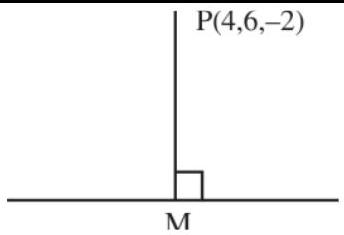
\includegraphics[max width=\textwidth, center]{2025_10_03_065db70bbae39307c94fg-5}

Equation of line is \(\frac{x+3}{3}=\frac{y-2}{3}=\frac{z-3}{-1}=\lambda\)\\
\(\mathrm{M}(3 \lambda-3,3 \lambda+2,3-\lambda)\)\\
D.R of \(\operatorname{PM}(3 \lambda-7,3 \lambda-4,5-\lambda)\)

Since PM is perpendicular to line\\
\(\Rightarrow 3(3 \lambda-7)+3(3 \lambda-4)-1(5-\lambda)=0\)\\
\(\Rightarrow \lambda=2\)\\
\(\Rightarrow \mathrm{M}(3,8,1) \Rightarrow \mathrm{PM}=\sqrt{14}\)\\
79. Let \(x, y, z>1\) and\\
\(\mathrm{A}=\left[\begin{array}{lll}1 & \log _{\mathrm{x}} \mathrm{y} & \log _{\mathrm{x}} \mathrm{z} \\ \log _{\mathrm{y}} \mathrm{x} & 2 & \log _{\mathrm{y}} \mathrm{z} \\ \log _{\mathrm{z}} \mathrm{x} & \log _{\mathrm{z}} \mathrm{y} & 3\end{array}\right]\).\\
Then \(\left|\operatorname{adj}\left(\operatorname{adj} \mathrm{A}^{2}\right)\right|\) is equal to\\
(1) \(6^{4}\)\\
(2) \(2^{8}\)\\
(3) \(4^{8}\)\\
(4) \(2^{4}\)

Official Ans. by NTA (2)\\
Allen Ans. (2)\\
Sol. \(|\mathrm{A}|=\frac{1}{\log \mathrm{x} \cdot \log \mathrm{y} \cdot \log \mathrm{z}}\left|\begin{array}{lll}\log \mathrm{x} & \log \mathrm{y} & \log \mathrm{z} \\ \log \mathrm{x} & 2 \log \mathrm{y} & \log \mathrm{z} \\ \log \mathrm{x} & \log \mathrm{y} & 3 \log \mathrm{z}\end{array}\right|=2\)\\
\(\Rightarrow\left|\operatorname{adj}\left(\operatorname{adj} \mathrm{A}^{2}\right)\right|=\left|\mathrm{A}^{2}\right|^{4}=2^{8}\)\\
80. If \(\mathrm{a}_{\mathrm{r}}\) is the coefficient of \(\mathrm{x}^{10-\mathrm{r}}\) in the Binomial expansion of \((1+x)^{10}\), then \(\sum_{r=1}^{10} r^{3}\left(\frac{a_{r}}{a_{r-1}}\right)^{2}\) is equal to\\
(1) 4895\\
(2) 1210\\
(3) 5445\\
(4) 3025

Official Ans. by NTA (2)\\
Allen Ans. (2)\\
Sol. \(\mathrm{a}_{\mathrm{r}}={ }^{10} \mathrm{C}_{10-\mathrm{r}}={ }^{10} \mathrm{C}_{\mathrm{r}}\)\\
\(\Rightarrow \sum_{\mathrm{r}=1}^{10} \mathrm{r}^{3}\left(\frac{{ }^{10} \mathrm{C}_{\mathrm{r}}}{{ }^{10} \mathrm{C}_{\mathrm{r}-1}}\right)^{2}=\sum_{\mathrm{r}=1}^{10} \mathrm{r}^{3}\left(\frac{11-\mathrm{r}}{\mathrm{r}}\right)^{2}=\sum_{\mathrm{r}=1}^{10} \mathrm{r}(11-\mathrm{r})^{2}\)\\
\(=\sum_{\mathrm{r}=1}^{10}\left(121 r+\mathrm{r}^{3}-22 \mathrm{r}^{2}\right)=1210\)

\section*{SECTION-B}
\begin{enumerate}
  \setcounter{enumi}{80}
  \item Let \(S=\{1,2,3,5,7,10,11\}\). The number of nonempty subsets of \(S\) that have the sum of all elements a multiple of 3 , is \(\_\_\_\_\) .
\end{enumerate}

\section*{Official Ans. by NTA (43)}
\section*{Allen Ans. (43)}
Sol. Elements of the type \(3 \mathrm{k}=3\)\\
Elements of the type \(3 \mathrm{k}+1=1,7,9\)\\
Elements of the type \(3 \mathrm{k}+2=2,5,11\)\\
Subsets containing one element \(\mathrm{S}_{1}=1\)\\
Subsets containing two elements\\
\(\mathrm{S}_{2}={ }^{3} \mathrm{C}_{1} \times{ }^{3} \mathrm{C}_{1}=9\)\\
Subsets containing three elements\\
\(\mathrm{S}_{3}={ }^{3} \mathrm{C}_{1} \times{ }^{3} \mathrm{C}_{1}+1+1=11\)

Subsets containing four elements\\
\(\mathrm{S}_{4}={ }^{3} \mathrm{C}_{3}+{ }^{3} \mathrm{C}_{3}+{ }^{3} \mathrm{C}_{2} \times{ }^{3} \mathrm{C}_{2}=11\)\\
Subsets containing five elements\\
\(\mathrm{S}_{5}={ }^{3} \mathrm{C}_{2} \times{ }^{3} \mathrm{C}_{2} \times 1=9\)\\
Subsets containing six elements \(\mathrm{S}_{6}=1\)\\
Subsets containing seven elements \(\mathrm{S}_{7}=1\)\\
\(\Rightarrow \operatorname{sum}=43\)\\
82. For some \(a, b, c \in \mathbb{N}\), let \(f(x)=a x-3\) and\\
\(g(x)=x^{b}+c, x \in \mathbb{R}\). If \((f \circ g)^{-1}(x)=\left(\frac{x-7}{2}\right)^{1 / 3}\), then \((\mathrm{fog})(\mathrm{ac})+(\mathrm{gof})(\mathrm{b})\) is equal to \(\_\_\_\_\) .

\section*{Official Ans. by NTA (2039)}
Allen Ans. (2039)\\
Sol. Let \(\operatorname{fog}(\mathrm{x})=\mathrm{h}(\mathrm{x})\)\\
\(\Rightarrow \mathrm{h}^{-1}(\mathrm{x})=\left(\frac{\mathrm{x}-7}{2}\right)^{\frac{1}{3}}\)\\
\(\Rightarrow \mathrm{h}(\mathrm{x})=\mathrm{fog}(\mathrm{x})=2 \mathrm{x}^{3}+7\)\\
\(\operatorname{fog}(\mathrm{x})=\mathrm{a}\left(\mathrm{x}^{\mathrm{b}}+\mathrm{c}\right)-3\)\\
\(\Rightarrow \mathrm{a}=2, \mathrm{~b}=3, \mathrm{c}=5\)\\
\(\Rightarrow \mathrm{fog}(\mathrm{ac})=\mathrm{fog}(10)=2007\)\\
\(g\left(f(x)=(2 x-3)^{3}+5\right.\)\\
\(\Rightarrow \operatorname{gof}(\mathrm{b})=\operatorname{gof}(3)=32\)\\
\(\Rightarrow\) sum \(=2039\)\\
83. The vertices of a hyperbola H are \(( \pm 6,0)\) and its eccentricity is \(\frac{\sqrt{5}}{2}\). Let N be the normal to H at a point in the first quadrant and parallel to the line \(\sqrt{2} x+y=2 \sqrt{2}\). If \(d\) is the length of the line segment of N between H and the y -axis then \(\mathrm{d}^{2}\) is equal to \(\_\_\_\_\) .

Official Ans. by NTA (216)\\
Allen Ans. (216)\\
Sol.\\
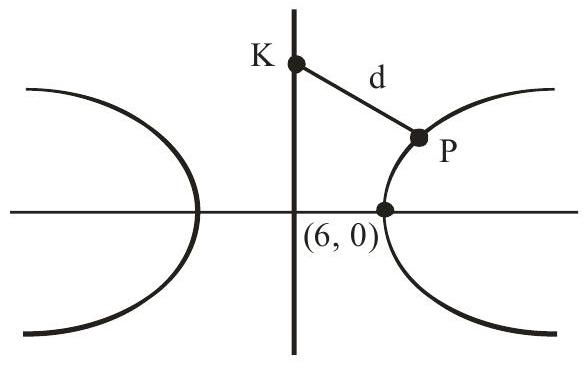
\includegraphics[max width=\textwidth, center]{2025_10_03_065db70bbae39307c94fg-6}\\
\(H: \frac{x^{2}}{36}-\frac{y^{2}}{9}=1\)\\
equation of normal is \(6 x \cos \theta+3 y \cot \theta=45\)\\
slope \(=-2 \sin \theta=-\sqrt{2}\)\\
\(\Rightarrow \theta=\frac{\pi}{4}\)

Equation of normal is \(\sqrt{2} x+y=15\)\\
\(\mathrm{P}:(\mathrm{a} \sec \theta, \mathrm{b} \tan \theta)\)\\
\(\Rightarrow \mathrm{P}(6 \sqrt{2}, 3)\) and \(\mathrm{K}(0,15)\)\\
\(\mathrm{d}^{2}=216\)\\
84. Let

\[
S=\left\{\alpha: \log _{2}\left(9^{2 \alpha-4}+13\right)-\log _{2}\left(\frac{5}{2} \cdot 3^{2 \alpha-4}+1\right)=2\right\} .
\]

Then the maximum value of \(\beta\) for which the equation \(x^{2}-2\left(\sum_{\alpha \in S} \alpha\right)^{2} x+\sum_{\alpha \in S}(\alpha+1)^{2} \beta=0\) has real roots, is \(\_\_\_\_\) -

\section*{Official Ans. by NTA (25)}
\section*{Allen Ans. (25)}
Sol. \(\quad \log _{2}\left(9^{2 \alpha-4}+13\right)-\log _{2}\left(\frac{5}{2} \cdot 3^{2 \alpha-4}+1\right)=2\)\\
\(\Rightarrow \frac{9^{2 \alpha-4}+13}{\frac{5}{2} 3^{2 \alpha-4}+1}=4\)\\
\(\Rightarrow \alpha=2 \quad\) or \(\quad 3\)\\
\(\sum_{\alpha \in S} \alpha=5\) and \(\sum_{\alpha \in S}(\alpha+1)^{2}=25\)\\
\(\Rightarrow \mathrm{x}^{2}-50 \mathrm{x}+25 \beta=0\) has real roots\\
\(\Rightarrow \beta \leq 25\)\\
\(\Rightarrow \beta_{\text {max }}=25\)\\
85. The constant term in the expansion of \(\left(2 x+\frac{1}{x^{7}}+3 x^{2}\right)^{5}\) is \(\_\_\_\_\) .

Official Ans. by NTA (1080)\\
Allen Ans. (1080)\\
Sol. General term is \(\sum \frac{5!(2 x)^{n_{1}}\left(x^{-7}\right)^{n_{2}}\left(3 x^{2}\right)^{n_{3}}}{n_{1}!n_{2}!n_{3}!}\)

For constant term,\\
\(\mathrm{n}_{1}+2 \mathrm{n}_{3}=7 \mathrm{n}_{2}\)\\
\& \(\mathrm{n}_{1}+\mathrm{n}_{2}+\mathrm{n}_{3}=5\)

Only possibility \(\mathrm{n}_{1}=1, \mathrm{n}_{2}=1, \mathrm{n}_{3}=3\)\\
\(\Rightarrow\) constant term \(=1080\)\\
86. Let \(\mathrm{A}_{1}, \mathrm{~A}_{2}, \mathrm{~A}_{3}\) be the three A.P. with the same common difference d and having their first terms as \(\mathrm{A}, \mathrm{A}+1, \mathrm{~A}+2\), respectively. Let \(\mathrm{a}, \mathrm{b}, \mathrm{c}\) be the \(7^{\text {th }}, 9^{\text {th }}, 17^{\text {th }}\) terms of \(\mathrm{A}_{1}, \mathrm{~A}_{2}, \mathrm{~A}_{3}\), respectively such that \(\left|\begin{array}{lll}\mathrm{a} & 7 & 1 \\ 2 \mathrm{~b} & 17 & 1 \\ \mathrm{c} & 17 & 1\end{array}\right|+70=0\)

If \(\mathrm{a}=29\), then the sum of first 20 terms of an AP whose first term is \(\mathrm{c}-\mathrm{a}-\mathrm{b}\) and common difference is \(\frac{\mathrm{d}}{12}\), is equal to \(\_\_\_\_\) .

Official Ans. by NTA (495)\\
Allen Ans. (495)\\
Sol. \(\left|\begin{array}{lll}A+6 d & 7 & 1 \\ 2(A+1+8 d) & 17 & 1 \\ A+2+16 d & 17 & 1\end{array}\right|+70=0\)\\
\(\Rightarrow \mathrm{A}=-7\) and \(\mathrm{d}=6\)\\
\(\therefore \mathrm{c}-\mathrm{a}-\mathrm{b}=20\)\\
\(\mathrm{S}_{20}=495\)\\
87. If the sum of all the solutions of\\
\(\tan ^{-1}\left(\frac{2 x}{1-x^{2}}\right)+\cot ^{-1}\left(\frac{1-x^{2}}{2 x}\right)=\frac{\pi}{3}\),\\
\(-1<x<1, x \neq 0\), is \(\alpha-\frac{4}{\sqrt{3}}\), then \(\alpha\) is equal to\\
\(\_\_\_\_\) .

\section*{Official Ans. by NTA (2)}
\section*{Allen Ans. (2)}
Sol. Case I : \(\mathrm{x}>0\)\\
\(\tan ^{-1} \frac{2 x}{1-x^{2}}+\tan ^{-1} \frac{2 x}{1-x^{2}}=\frac{\pi}{3}\)\\
\(\mathrm{x}=2-\sqrt{3}\)\\
Case II : \(\mathrm{x}<0\)\\
\(\tan ^{-1} \frac{2 x}{1-x^{2}}+\tan ^{-1} \frac{2 x}{1-x^{2}}+\pi=\frac{\pi}{3}\)\\
\(\mathrm{x}=\frac{-1}{\sqrt{3}} \Rightarrow \alpha=2\)\\
88. Let the equation of the plane passing through the line\\
\(x-2 y-z-5=0=x+y+3 z-5\) and parallel to the line \(\mathrm{x}+\mathrm{y}+2 \mathrm{z}-7=0=2 \mathrm{x}+3 \mathrm{y}+\mathrm{z}-2\) be \(\mathrm{ax}+\mathrm{by}+\mathrm{cz}=65\). Then the distance of the point \((\mathrm{a}, \mathrm{b}, \mathrm{c})\) from the plane \(2 \mathrm{x}+2 \mathrm{y}-\mathrm{z}+16=0\) is\\
\(\_\_\_\_\) .

Official Ans. by NTA (9)\\
Allen Ans. (9)\\
Sol. Equation of plane is\\
\((x-2 y-z-5)+b(x+y+3 z-5)=0\)\\
\(\left|\begin{array}{lll}1+\mathrm{b} & -2+\mathrm{b} & -1+3 \mathrm{~b} \\ 1 & 1 & 2 \\ 2 & 3 & 1\end{array}\right|=0\)\\
\(\Rightarrow \mathrm{b}=12\)\\
\(\therefore\) plane is \(13 x+10 y+35 z=65\)\\
Distance from given point to plane \(=9\)\\
89. Let x and y be distinct integers where \(1 \leq \mathrm{x} \leq 25\) and \(1 \leq y \leq 25\). Then, the number of ways of choosing x and y , such that \(\mathrm{x}+\mathrm{y}\) is divisible by 5 , is \(\_\_\_\_\) .

Official Ans. by NTA (120)\\
Allen Ans. (120)\\
Sol. \(x+y=5 \lambda\)

\section*{Cases :}
\begin{center}
\begin{tabular}{llc}
\(\mathbf{x}\) & \(\mathbf{y}\) & Number of ways \\
\(5 \lambda\) & \(5 \lambda\) & 20 \\
\(5 \lambda+1\) & \(5 \lambda+4\) & 25 \\
\(5 \lambda+2\) & \(5 \lambda+3\) & 25 \\
\(5 \lambda+3\) & \(5 \lambda+2\) & 25 \\
\(5 \lambda+4\) & \(5 \lambda+1\) & 25 \\
\end{tabular}
\end{center}

Total = 120\\
90. It the area enclosed by the parabolas \(P_{1}: 2 y=5 x^{2}\) and \(P_{2}: x^{2}-y+6=0\) is equal to the area enclosed by \(P_{1}\) and \(y=\alpha x, \alpha>0\), then \(\alpha^{3}\) is equal to\\
\(\_\_\_\_\) .

Official Ans. by NTA (600)\\
Allen Ans. (600)\\
Sol.\\
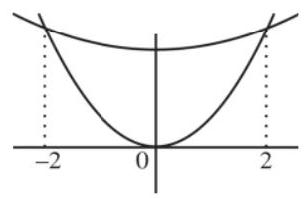
\includegraphics[max width=\textwidth, center]{2025_10_03_065db70bbae39307c94fg-8}

Abscissa of point of intersection of \(2 y=5 x^{2}\) and \(y=x^{2}+6\) is \(\pm 2\)\\
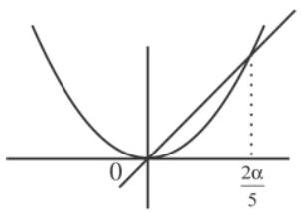
\includegraphics[max width=\textwidth, center]{2025_10_03_065db70bbae39307c94fg-8(1)}

Area \(=2 \int_{0}^{2}\left(x^{2}+6-\frac{5 x^{2}}{2}\right) d x=\int_{0}^{\frac{2 \alpha}{5}}\left(\alpha x-\frac{5 x^{2}}{2}\right) d x\)\\
\(\Rightarrow \int_{0}^{\frac{2 \alpha}{5}}\left(\alpha x-\frac{5 x^{2}}{2}\right) d x=16\)\\
\(\Rightarrow \alpha^{3}=600\)


\end{document}